% ----------------------------------------------------
% System Testing
% ----------------------------------------------------
\documentclass[class=report,11pt,crop=false]{standalone}
% Page geometry
\usepackage[a4paper,margin=20mm,top=25mm,bottom=25mm]{geometry}

% Font choice
\usepackage{lmodern}

% Use IEEE bibliography style
\bibliographystyle{IEEEtran}

% Line spacing
\usepackage{setspace}
\setstretch{1.20}

% Ensure UTF8 encoding
\usepackage[utf8]{inputenc}

% Language standard (not too important)
\usepackage[english]{babel}

% Skip a line in between paragraphs
\usepackage{parskip}

% For the creation of dummy text
\usepackage{blindtext}

% Math
\usepackage{amsmath}

% Header & Footer stuff
\usepackage{fancyhdr}
\pagestyle{fancy}
\fancyhead{}
\fancyhead[R]{\nouppercase{\rightmark}}
\fancyfoot{}
\fancyfoot[C]{\thepage}
\renewcommand{\headrulewidth}{0.0pt}
\renewcommand{\footrulewidth}{0.0pt}
\setlength{\headheight}{13.6pt}

% Epigraphs
\usepackage{epigraph}
\setlength\epigraphrule{0pt}
\setlength{\epigraphwidth}{0.65\textwidth}

% Colour
\usepackage{color}
\usepackage[usenames,dvipsnames]{xcolor}

% Hyperlinks & References
\usepackage{hyperref}
\definecolor{linkColour}{RGB}{77,71,179}
\hypersetup{
    colorlinks=true,
    linkcolor=linkColour,
    filecolor=linkColour,
    urlcolor=linkColour,
    citecolor=linkColour,
}
\urlstyle{same}

% Automatically correct front-side quotes
\usepackage[autostyle=false, style=ukenglish]{csquotes}
\MakeOuterQuote{"}

% Graphics
\usepackage{graphicx}
\graphicspath{{Images/}{../Images/}}
\usepackage{makecell}
\usepackage{transparent}

% SI units
\usepackage{siunitx}

% Microtype goodness
\usepackage{microtype}

% Listings
\usepackage[T1]{fontenc}
\usepackage{listings}
\usepackage[scaled=0.8]{DejaVuSansMono}

% Custom colours for listings
\definecolor{backgroundColour}{RGB}{250,250,250}
\definecolor{commentColour}{RGB}{73, 175, 102}
\definecolor{identifierColour}{RGB}{196, 19, 66}
\definecolor{stringColour}{RGB}{252, 156, 30}
\definecolor{keywordColour}{RGB}{50, 38, 224}
\definecolor{lineNumbersColour}{RGB}{127,127,127}
\lstset{
  language=Matlab,
  captionpos=b,
  aboveskip=15pt,belowskip=10pt,
  backgroundcolor=\color{backgroundColour},
  basicstyle=\ttfamily,%\footnotesize,        % the size of the fonts that are used for the code
  breakatwhitespace=false,         % sets if automatic breaks should only happen at whitespace
  breaklines=true,                 % sets automatic line breaking
  postbreak=\mbox{\textcolor{red}{$\hookrightarrow$}\space},
  commentstyle=\color{commentColour},    % comment style
  identifierstyle=\color{identifierColour},
  stringstyle=\color{stringColour},
   keywordstyle=\color{keywordColour},       % keyword style
  %escapeinside={\%*}{*)},          % if you want to add LaTeX within your code
  extendedchars=true,              % lets you use non-ASCII characters; for 8-bits encodings only, does not work with UTF-8
  frame=single,	                   % adds a frame around the code
  keepspaces=true,                 % keeps spaces in text, useful for keeping indentation of code (possibly needs columns=flexible)
  morekeywords={*,...},            % if you want to add more keywords to the set
  numbers=left,                    % where to put the line-numbers; possible values are (none, left, right)
  numbersep=5pt,                   % how far the line-numbers are from the code
  numberstyle=\tiny\color{lineNumbersColour}, % the style that is used for the line-numbers
  rulecolor=\color{black},         % if not set, the frame-color may be changed on line-breaks within not-black text (e.g. comments (green here))
  showspaces=false,                % show spaces everywhere adding particular underscores; it overrides 'showstringspaces'
  showstringspaces=false,          % underline spaces within strings only
  showtabs=false,                  % show tabs within strings adding particular underscores
  stepnumber=1,                    % the step between two line-numbers. If it's 1, each line will be numbered
  tabsize=2,	                   % sets default tabsize to 2 spaces
  %title=\lstname                   % show the filename of files included with \lstinputlisting; also try caption instead of title
}

% Caption stuff
\usepackage[hypcap=true, justification=centering]{caption}
\usepackage{subcaption}

% Glossary package
% \usepackage[acronym]{glossaries}
\usepackage{glossaries-extra}
\setabbreviationstyle[acronym]{long-short}

% For Proofs & Theorems
\usepackage{amsthm}

% Maths symbols
\usepackage{amssymb}
\usepackage{mathrsfs}
\usepackage{mathtools}

% For algorithms
\usepackage[]{algorithm2e}

% Spacing stuff
\setlength{\abovecaptionskip}{5pt plus 3pt minus 2pt}
\setlength{\belowcaptionskip}{5pt plus 3pt minus 2pt}
\setlength{\textfloatsep}{10pt plus 3pt minus 2pt}
\setlength{\intextsep}{15pt plus 3pt minus 2pt}

% For aligning footnotes at bottom of page, instead of hugging text
\usepackage[bottom]{footmisc}

% Add LoF, Bib, etc. to ToC
\usepackage[nottoc]{tocbibind}

% SI
\usepackage{siunitx}

% For removing some whitespace in Chapter headings etc
\usepackage{etoolbox}
\makeatletter
\patchcmd{\@makechapterhead}{\vspace*{50\p@}}{\vspace*{-10pt}}{}{}%
\patchcmd{\@makeschapterhead}{\vspace*{50\p@}}{\vspace*{-10pt}}{}{}%
\makeatother
\makenoidxglossaries
% --------------------------------------------------------------------
% Examples of creating a glossary
\newacronym{cw}{CW}{Continuous-Wave}
\newacronym{dsp}{DSP}{Digital Signal Processing}
\newacronym{em}{EM}{Electromagnetic}
\newacronym{fmcw}{FMCW}{Frequency Modulated Continuous Wave}
\newacronym{gui}{GUI}{Graphical User Interface}
\newacronym{rf}{RF}{Radio Frequency}
\newacronym{radar}{RADAR}{Radio Detection and Ranging}
\newacronym{pcb}{PCB}{Printed Circuit Board}
\newacronym{pc}{PC}{Personal Computer}
\newacronym{pri}{PRI}{Pulse Repetition Interval}
\newacronym{adc}{ADC}{Analogue-to-Digital Converter}
\newacronym{if}{IF}{Intermediate Frequency}
\newacronym{itu}{ITU}{International Telecommunications Union}
\newacronym{rcs}{RCS}{Radar Cross Section}
\newacronym{opamp}{Op Amp}{Operational Amplifier}
\newacronym{gbwp}{GBWP}{Gain Bandwidth Product}
\newacronym{dc}{DC}{Direct Current}
\newacronym{ac}{AC}{Alternating Current}
\newacronym{uct}{UCT}{University of Cape Town}
\newacronym{usb}{USB}{Universal Serial Bus}
\newacronym{stft}{STFT}{Short-Time Fourier Transform}
\newacronym{fft}{FFT}{Fast Fourier Transform}
\newacronym{dft}{DFT}{Discrete Fourier Transform}
\newacronym{dtft}{DTFT}{Discrete-Time Fourier Transform}
\newacronym{snr}{SNR}{Signal-to-Noise Ratio}
\newacronym{prf}{PRF}{Pulse Repetition Frequency}
\newacronym{isar}{ISAR}{Inverse Synthetic Aperture}
% include SUV (check experimentation table)
% --------------------------------------------------------------------

\begin{document}
% ----------------------------------------------------
\chapter{System Testing \label{ch:testing}}
\vspace{-1cm}
% ----------------------------------------------------
This chapter details the tests performed on each sub-system to ensure its performance is in alliance with the requirements of the design. Each sub-system is first tested in simulation before the built hardware is tested to ensure it matches up to the simulated results. The hardware then undergoes some tests once the transmitter and receiver circuits are integrated - this is to validate that the integrated system works as desired.

%\section{Ultrasonic Transducer}

\section{Transmitter Circuit}
Figure~\ref{fig:transmitter-circuit} shows the LTSpice model of the transmitter circuit.  

\begin{figure}[htbp]
    \centering
    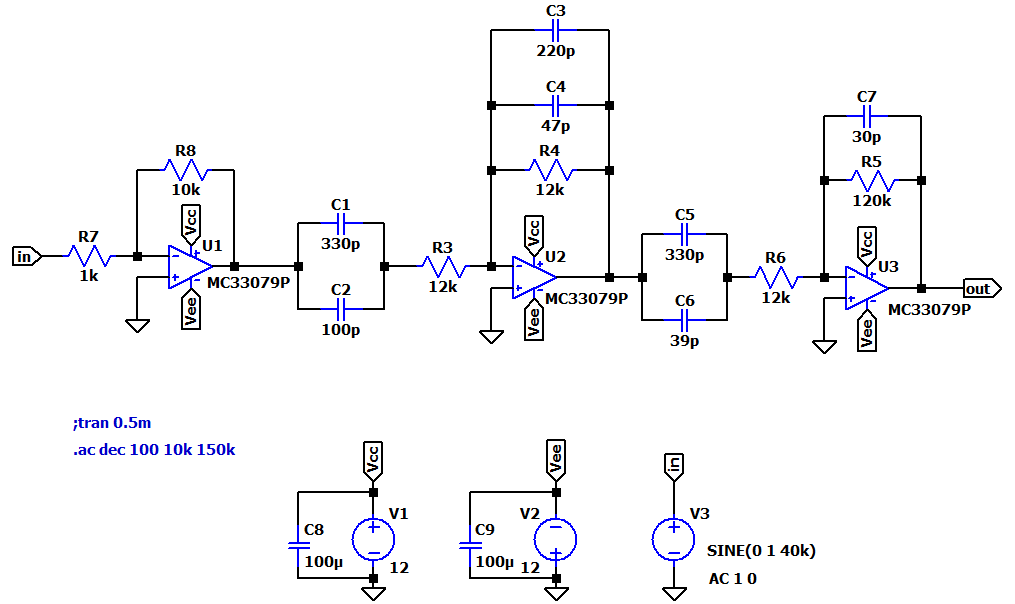
\includegraphics[width=0.8\columnwidth]{../Images/transmitter_circuit_diagram.png}
    \caption{Transmitter circuit}
    \label{fig:transmitter-circuit}
\end{figure}

\subsection{Simulations}\label{sect:transmitter-simulations}
The amplifier was designed to produce a linear gain of 10, hence, the input signal should be amplified by a factor of 10. Figure~\ref{fig:signal-amplifier} shows the results of the simulated signal amplifier. A transient analysis was run with an input signal of 1 V; this resulted in a 10 V output signal. This lines up with the expectations of the design. The physical hardware will be adjustable, so the amplifier will be able to amplify the input signal to variable voltages up to a factor of 10.

% signal amplifier
\begin{figure}[htbp]
    \centering
    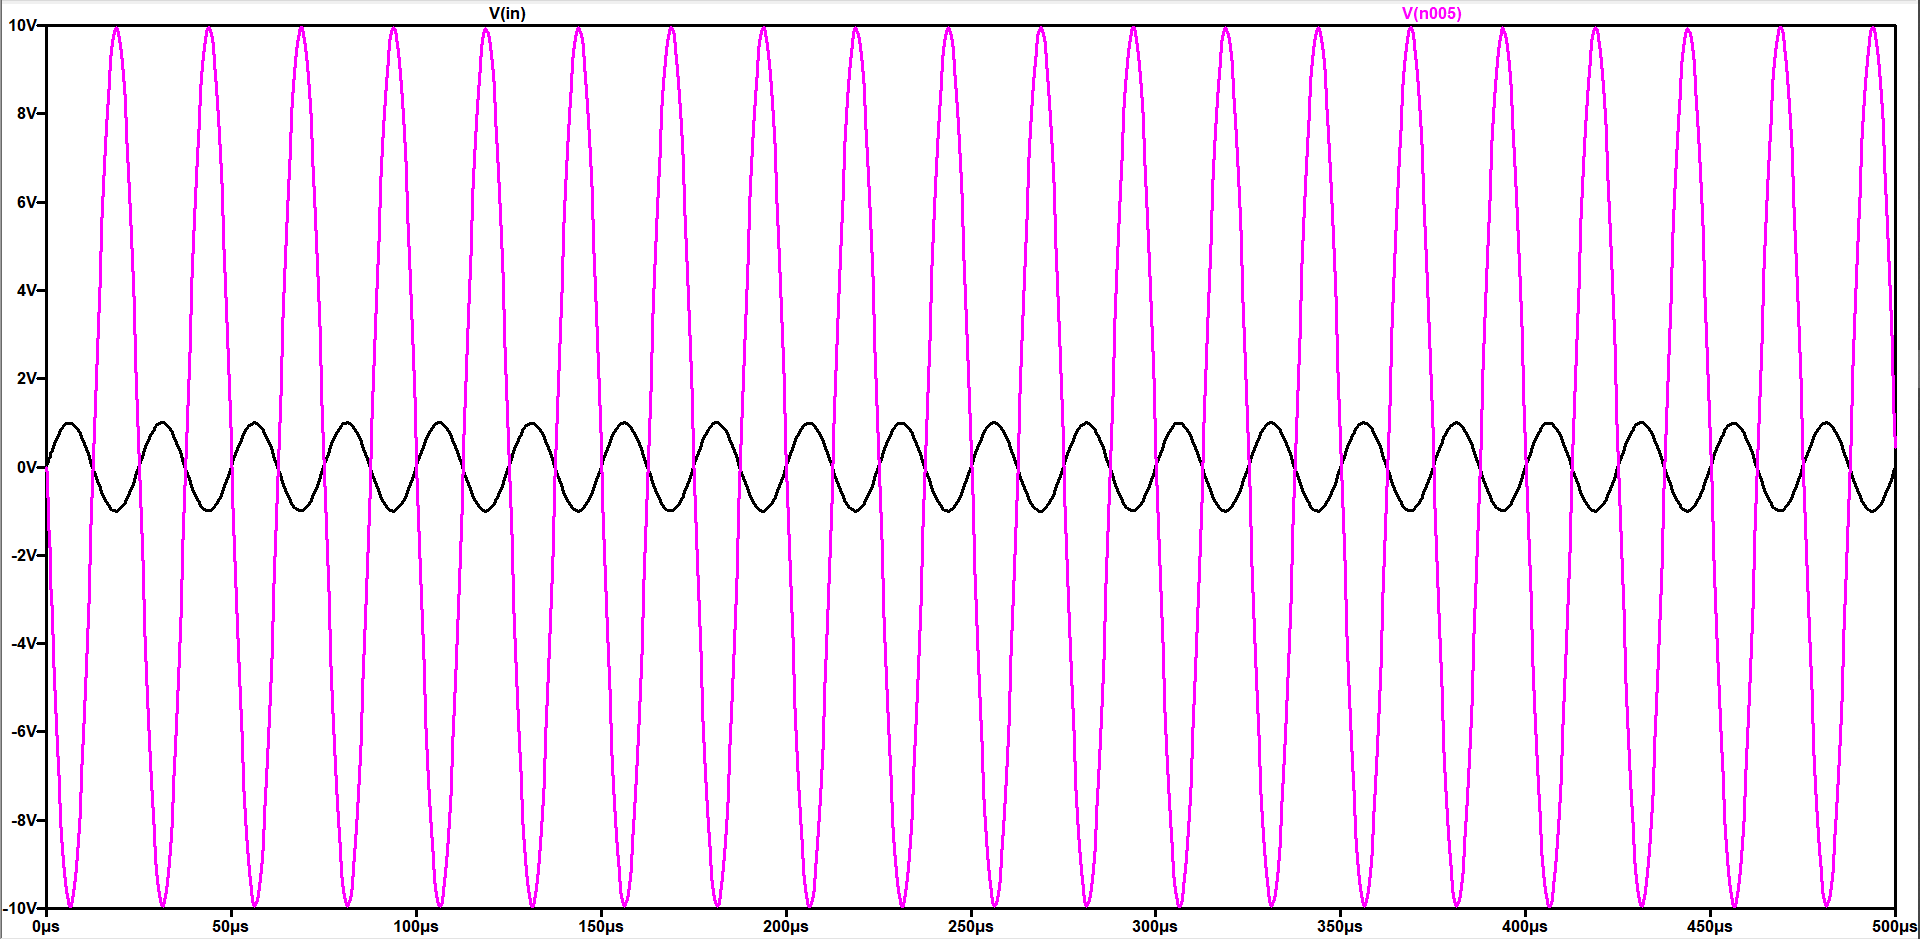
\includegraphics[width=0.8\columnwidth]{../Images/sim/amplifier_simulation.png}
    \caption{Signal amplifier simulation}
    \label{fig:signal-amplifier}
\end{figure}

The two-stage filter was designed to filter out signals outside the range of 30 kHz to 50 kHz for the first stage, and 36 kHz and 44 kHz for the second stage. An AC analysis was run to evaluate the frequency response. The frequency response of the first stage, shown in Figure~\ref{fig:filter-stage-1}, shows that the response is centered at 38.8 kHz with cutoff frequencies of 15.9 kHz for $f_L$ and 95.3 kHz for $f_H$. The second stage, shown in Figure~\ref{fig:filter-stage-2}, shows that the response is centered at 38.7 kHz with cutoff frequencies of 21.2 kHz for $f_L$ and 71.6 kHz for $f_H$. The results of the simulations for both stages do not match up very closely with the calculations made in Chapter~\ref{ch:design} section, but produce a centered frequency that is agreeable with the 40 kHz requirement. Although the simulations result in a frequency range of 21.2 kHz to 71.6 kHz, it is expected that the narrow bandwidth of the ultrasonic barrel transmitter should be able to attenuate the transmitted signals outside its bandwidth of approximately $\pm$3 kHz.

% two-stage band-pass filter
\begin{figure}[htbp]
    \centering
    \captionsetup{type=figure}
    \begin{subfigure}[t]{0.45\textwidth}
        \centering
        \def\svgwidth{1\linewidth}
        {\scriptsize
            \setstretch{0.7} % Line spacing
            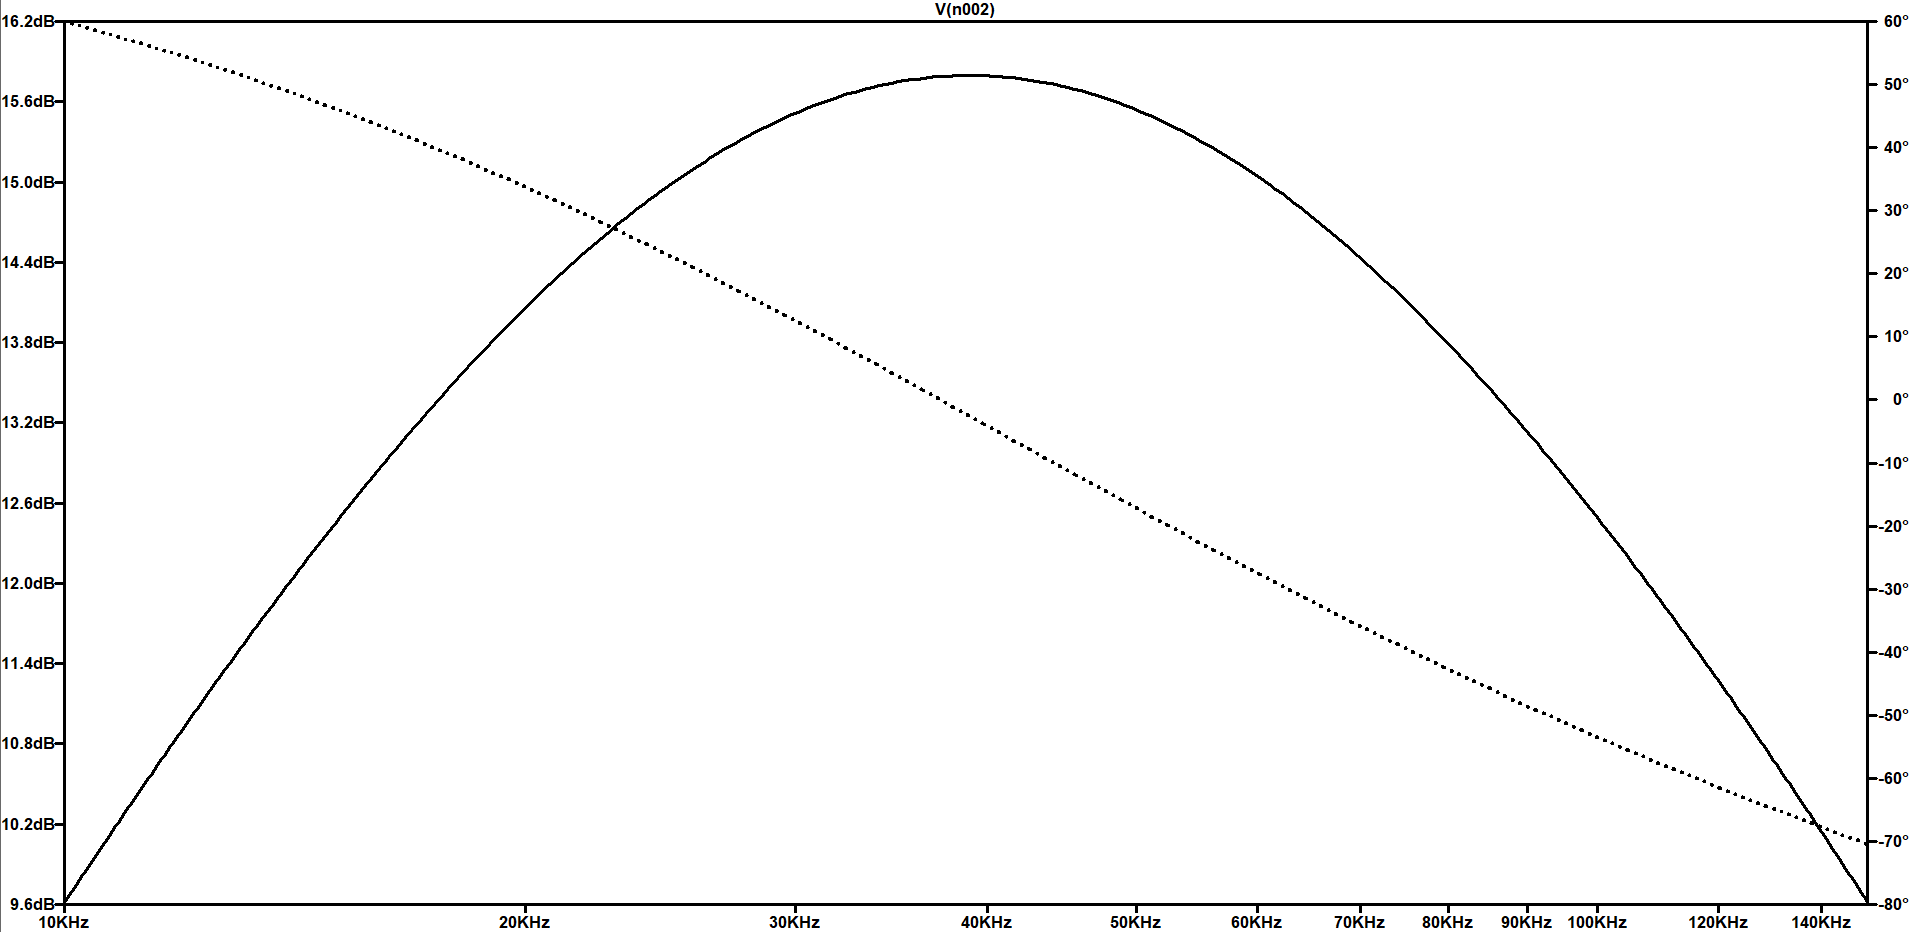
\includegraphics[width=8.5cm,height=6cm]{../Images/sim/filter_stage_1.png}}
        \caption{First stage of band-pass filter.}
        \label{fig:filter-stage-1}
    \end{subfigure}%
    ~ 
    \begin{subfigure}[t]{0.5\textwidth}
        \def\svgwidth{1\linewidth}
        {\scriptsize
            \setstretch{0.7} % Line spacing
            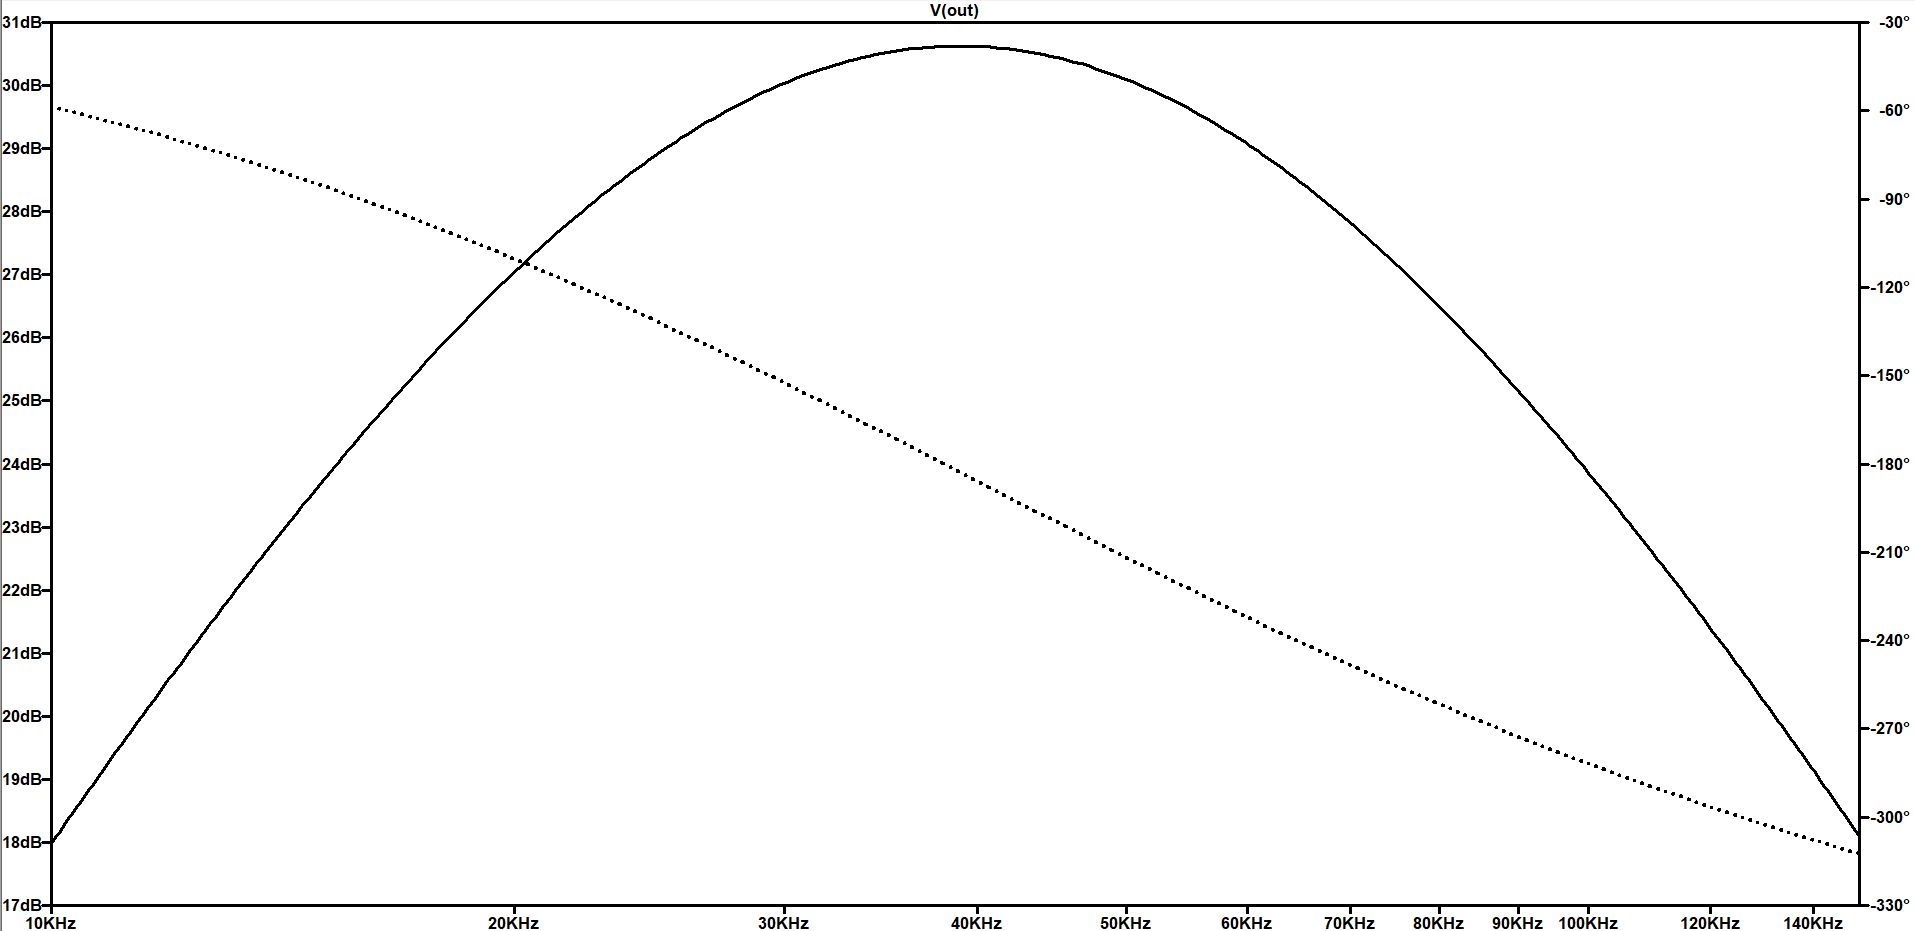
\includegraphics[width=8.5cm,height=6cm]{../Images/sim/filter_stage_2.png}}
        \caption{Second stage of band-pass filter.}
        \label{fig:filter-stage-2}
    \end{subfigure}
    \caption{Simulated frequency response of the two-stage band-pass filter.}
    \label{fig:band-pass-filter-simulations}
\end{figure}

\subsection{Hardware}
Figure~\ref{fig:osc-transmitter-1} shows the oscilloscope readings for the input signal to the transmitter circuit (Figure~\ref{fig:osc-transmitter-input}) and the output of the amplifier (Figure~\ref{fig:osc-transmitter-amplifier}). A 2 $V_p_p$ signal with 40 kHz frequency is used as the input to the transmitter using a signal generator. The potentiometer is then adjusted to provide a linear gain of 10. The figure shows that the input signal is 1.8 $V_p_p$ with a 40 kHz frequency and outputs 10 V$V_p_p$ at the same frequency. These results are agreeable with the simulation and the design calculations.

% input signal and amplified signal
\begin{figure}[htbp]
    \centering
    \captionsetup{type=figure}
    \begin{subfigure}[t]{0.5\textwidth}
        \centering
        \def\svgwidth{1\linewidth}
        {\scriptsize
            \setstretch{0.7} % Line spacing
            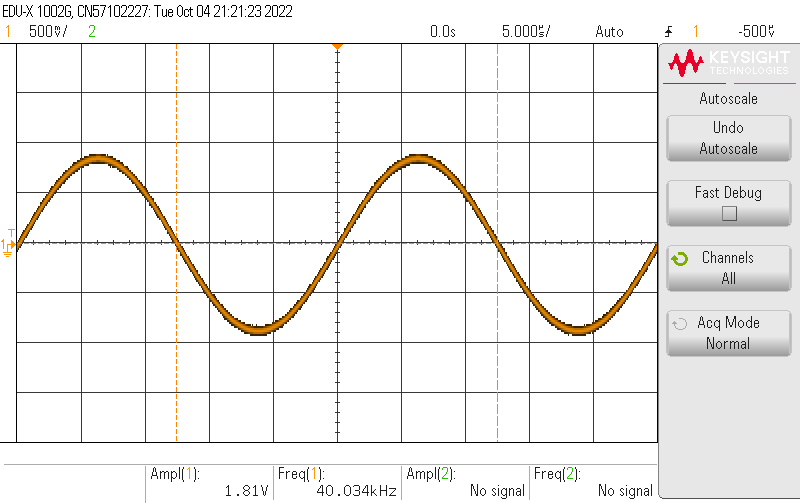
\includegraphics[width=8.5cm,height=6cm]{../Images/scope_1.png}}
        \caption{Input signal to the transmitter.}
        \label{fig:osc-transmitter-input}
    \end{subfigure}%
    ~ 
    \begin{subfigure}[t]{0.5\textwidth}
        \def\svgwidth{1\linewidth}
        {\scriptsize
            \setstretch{0.7} % Line spacing
            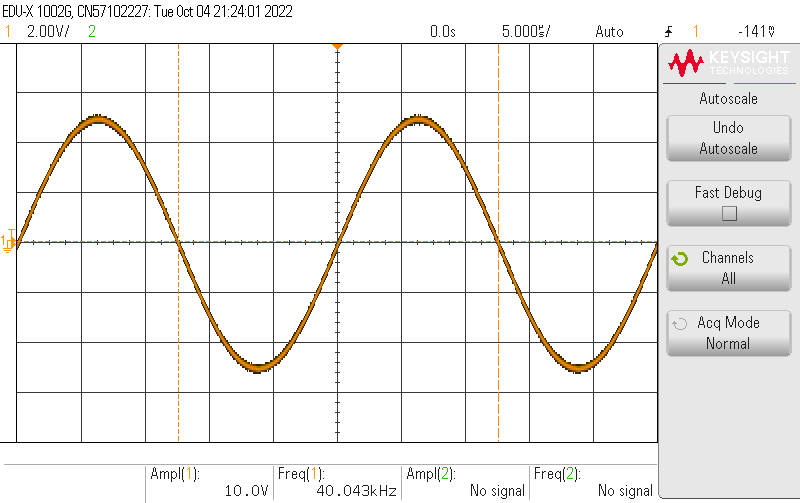
\includegraphics[width=8.5cm,height=6cm]{../Images/scope_2.png}}
        \caption{Amplified signal.}
        \label{fig:osc-transmitter-amplifier}
    \end{subfigure}
    \caption{Oscilloscope readings of the input signal and amplified signal of the transmitter.}
    \label{fig:osc-transmitter-1}
\end{figure}

Figure~\ref{fig:osc-transmitter-2} shows the oscilloscope readings of the output of each stage of the bandpass filter. Figure~\ref{fig:osc-transmitter-bpf-1} and Figure~\ref{fig:osc-transmitter-bpf-2} show that the frequency response is centered at 40 kHz; these results validate the results of the simulations and design specifications.

% bandpass filter
\begin{figure}[htbp]
    \centering
    \captionsetup{type=figure}
    \begin{subfigure}[t]{0.5\textwidth}
        \centering
        \def\svgwidth{1\linewidth}
        {\scriptsize
            \setstretch{0.7} % Line spacing
            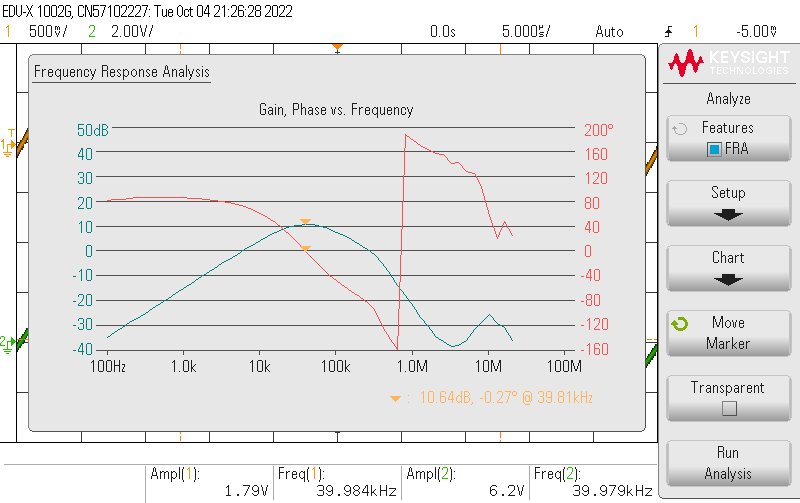
\includegraphics[width=8.5cm,height=6cm]{../Images/scope_4.png}}
        \caption{First stage of band-pass filter.}
        \label{fig:osc-transmitter-bpf-1}
    \end{subfigure}%
    ~ 
    \begin{subfigure}[t]{0.5\textwidth}
        \def\svgwidth{1\linewidth}
        {\scriptsize
            \setstretch{0.7} % Line spacing
            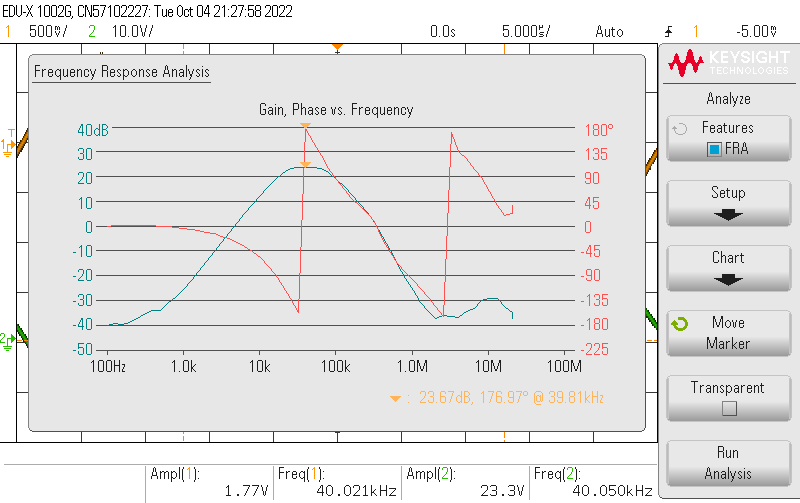
\includegraphics[width=8.5cm,height=6cm]{../Images/scope_6.png}}
        \caption{Second stage of band-pass filter.}
        \label{fig:osc-transmitter-bpf-2}
    \end{subfigure}
    \caption{Oscilloscope frequency response of the two-stage band-pass filter.}
    \label{fig:osc-transmitter-2}
\end{figure}

\section{Receiver Circuit}
Figure~\ref{fig:receiver-circuit} shows the LTSpice model of the receiver circuit.  

\begin{figure}[htbp]
    \centering
    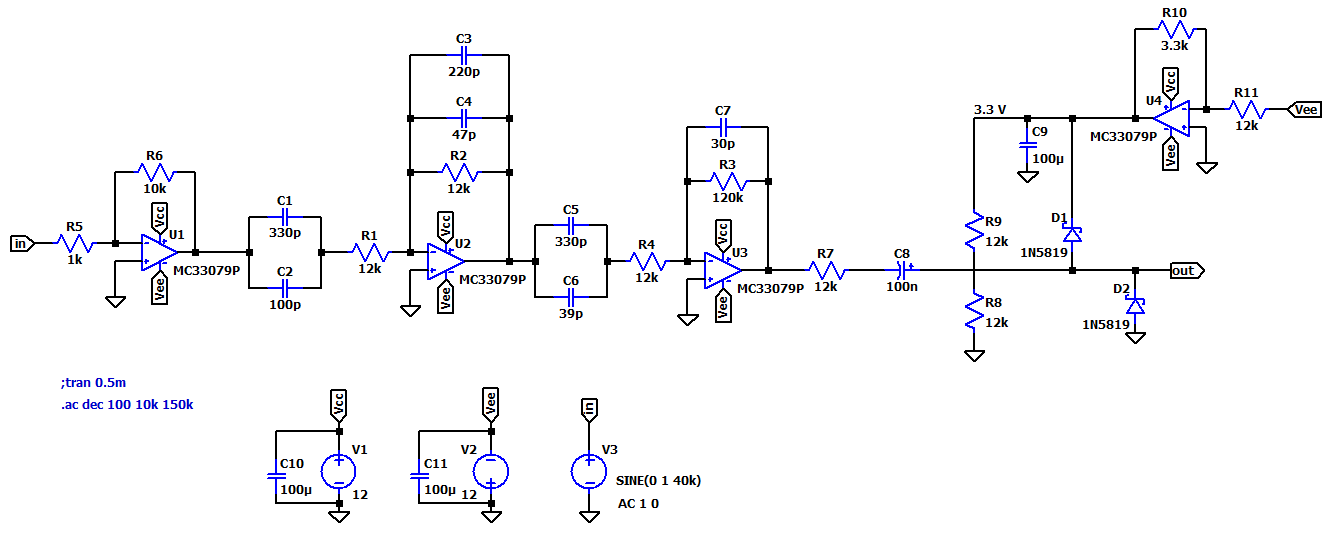
\includegraphics[width=0.8\columnwidth]{../Images/receiver_circuit_diagram.png}
    \caption{Receiver circuit}
    \label{fig:receiver-circuit}
\end{figure}

\subsection{Simulations}
The receiver circuit contains a signal amplifier and bandpass filter identical to that designed for the transmitter. The receiver will therefore produce the same results in simulations as that provided in Section~\ref{sect:transmitter-simulations}. In \textsc{LTSpice}, a transient analysis was run to simulate the ouput of the op-amp that produces the 3.3 V signal and the overall output of the receiver circuit. The simulated results are shown in Figure~\ref{fig:receiver-output-simulation}. The figure shows a horizontal black line at about 3.3 V - this is the DC signal produces by the op-amp U4. The simulation shows that the receiver outputs a signal that has been clamped to oscillate above approximately -0.2 V and is clipped to approximately 3.45 V. These values are not identical to the calculations but produce very accurate results and are therefore good results. Practically, the potentiometer will be turned to ensure the output is no more than 3.3 V and it is expected that the XONAR U5 is able to handle the small negative voltage.  

\begin{figure}[htbp]
    \centering
    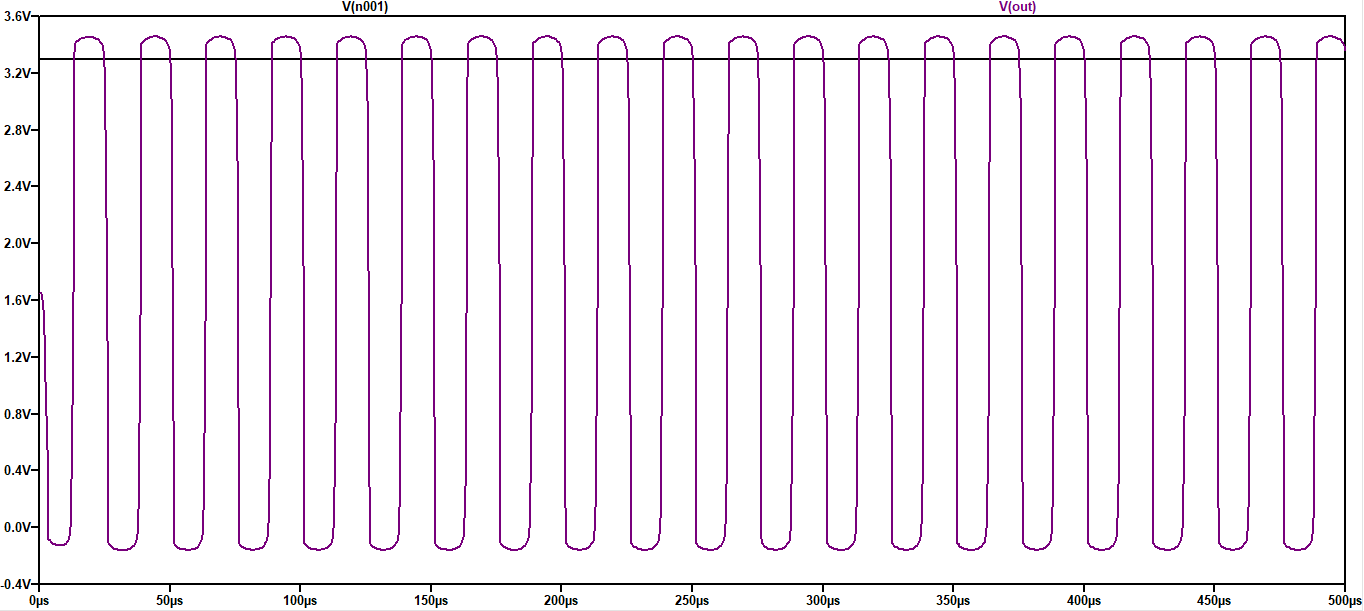
\includegraphics[width=0.8\columnwidth]{../Images/sim/receiver_simulation.png}
    \caption{Output of the receiver circuit}
    \label{fig:receiver-output-simulation}
\end{figure}

\subsection{Hardware}
For the hardware testing of the receiver circuit, it was important to test every part of the circuit to ensure it operates correctly. Although the amplifier and bandpass filter would expectantly produce similar results in simulation, it is expected that there will be practical differences observable with the built hardware.
Figure~\ref{fig:osc-receiver-1} shows the oscilloscope readings for the input signal to the receiver circuit (Figure~\ref{fig:osc-receiver-input}) and the output of the amplifier (Figure~\ref{fig:osc-receiver-amplifier}). A 2 $V_p_p$ signal with 40 kHz frequency is used as the input to the transmitter using a signal generator. The potentiometer is then adjusted to provide a linear gain of 10. The figure shows that the input signal is 1.91 $V_p_p$ with a 40 kHz frequency and outputs 10 V$V_p_p$ at the same frequency. Although the 10 V$V_p_p$ amplified signal validates the design calculations and simulations, the readings show that the amplified signal is clipped to 3.62 V instead of producing a 5 V amplitude. 

% input signal and amplified signal
\begin{figure}[htbp]
    \centering
    \captionsetup{type=figure}
    \begin{subfigure}[t]{0.5\textwidth}
        \centering
        \def\svgwidth{1\linewidth}
        {\scriptsize
            \setstretch{0.7} % Line spacing
            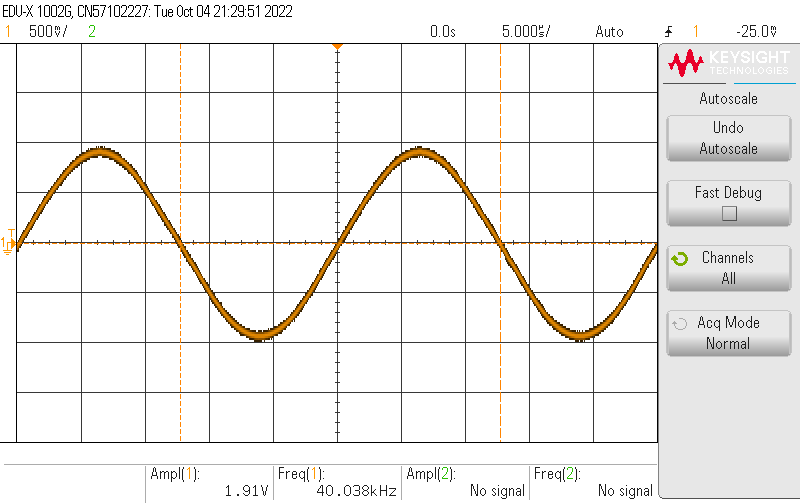
\includegraphics[width=8.5cm,height=6cm]{../Images/scope_7.png}}
        \caption{Input signal to the receiver.}
        \label{fig:osc-receiver-input}
    \end{subfigure}%
    ~ 
    \begin{subfigure}[t]{0.5\textwidth}
        \def\svgwidth{1\linewidth}
        {\scriptsize
            \setstretch{0.7} % Line spacing
            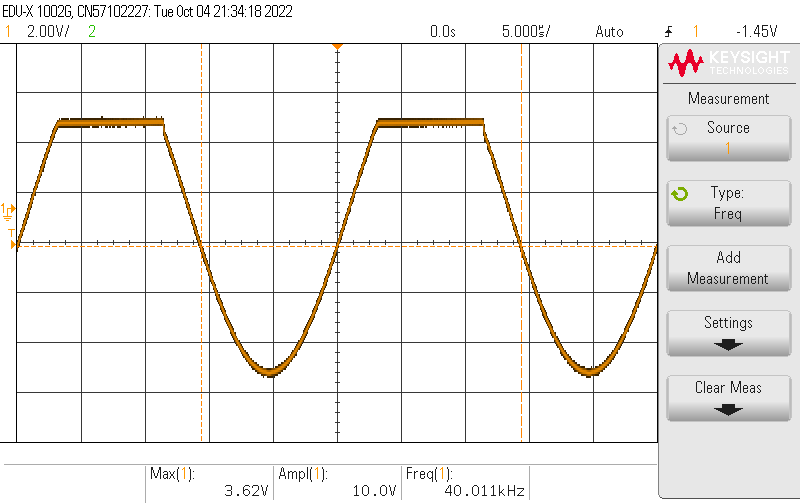
\includegraphics[width=8.5cm,height=6cm]{../Images/scope_8.png}}
        \caption{Amplified signal.}
        \label{fig:osc-receiver-amplifier}
    \end{subfigure}
    \caption{Oscilloscope readings of the input signal and amplified signal of the receiver.}
    \label{fig:osc-receiver-1}
\end{figure}

Figure~\ref{fig:osc-receiver-2} shows the oscilloscope readings of the output of each stage of the bandpass filter. Figure~\ref{fig:osc-receiver-bpf-1} and Figure~\ref{fig:osc-receiver-bpf-2} show that the frequency response is centered at 40 kHz; these results validate the results of the simulations and design specifications.

% bandpass filter
\begin{figure}[htbp]
    \centering
    \captionsetup{type=figure}
    \begin{subfigure}[t]{0.5\textwidth}
        \centering
        \def\svgwidth{1\linewidth}
        {\scriptsize
            \setstretch{0.7} % Line spacing
            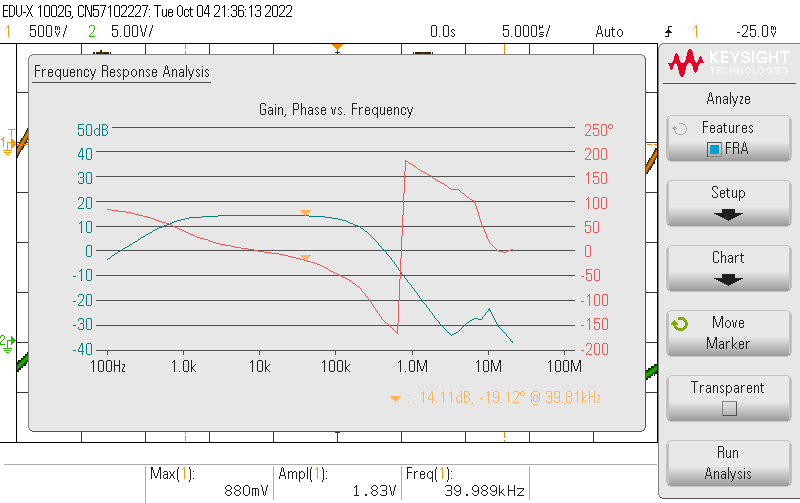
\includegraphics[width=8.5cm,height=6cm]{../Images/scope_10.png}}
        \caption{First stage of band-pass filter.}
        \label{fig:osc-receiver-bpf-1}
    \end{subfigure}%
    ~ 
    \begin{subfigure}[t]{0.5\textwidth}
        \def\svgwidth{1\linewidth}
        {\scriptsize
            \setstretch{0.7} % Line spacing
            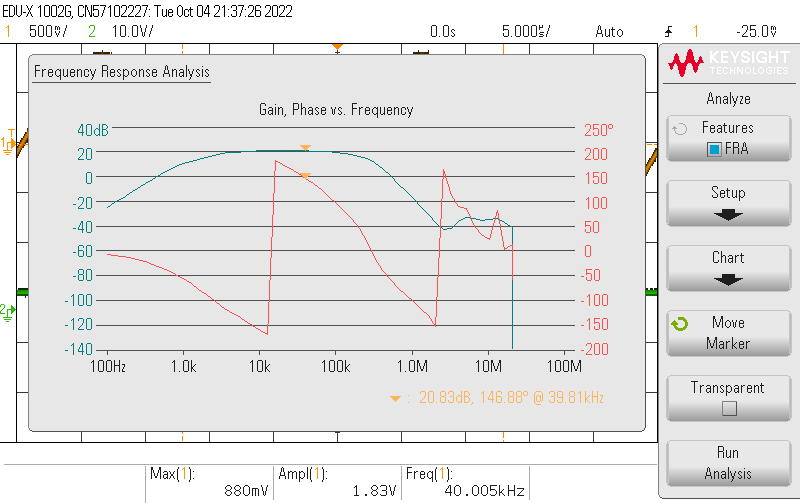
\includegraphics[width=8.5cm,height=6cm]{../Images/scope_12.png}}
        \caption{Second stage of band-pass filter.}
        \label{fig:osc-receiver-bpf-2}
    \end{subfigure}
    \caption{Oscilloscope frequency response of the two-stage band-pass filter.}
    \label{fig:osc-receiver-2}
\end{figure}

Figure~\ref{fig:osc-receiver-2} shows the oscilloscope readings of the 3.3 V DC signal generated by the op-amp and the output signal of the receiver circuit. Figure~\ref{fig:osc-receiver-3-3} shows that the signal actually outputs 3.6 V instead of 3.3 V; this is not an issue because the signal is further clamped and clipped accurately to 3.3 V using the potentiometer, as shown in Figure\ref{fig:osc-receiver-clamp-clip}.

% 3.3 V and clipped and clamped signal
\begin{figure}[htbp]
    \centering
    \captionsetup{type=figure}
    \begin{subfigure}[t]{0.5\textwidth}
        \centering
        \def\svgwidth{1\linewidth}
        {\scriptsize
            \setstretch{0.7} % Line spacing
            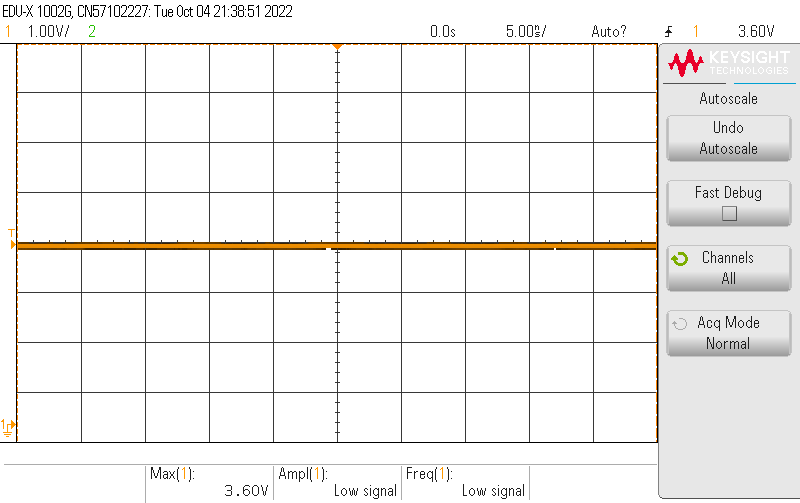
\includegraphics[width=8.5cm,height=6cm]{../Images/scope_14.png}}
        \caption{3.3 V generated signal.}
        \label{fig:osc-receiver-3-3}
    \end{subfigure}%
    ~ 
    \begin{subfigure}[t]{0.5\textwidth}
        \def\svgwidth{1\linewidth}
        {\scriptsize
            \setstretch{0.7} % Line spacing
            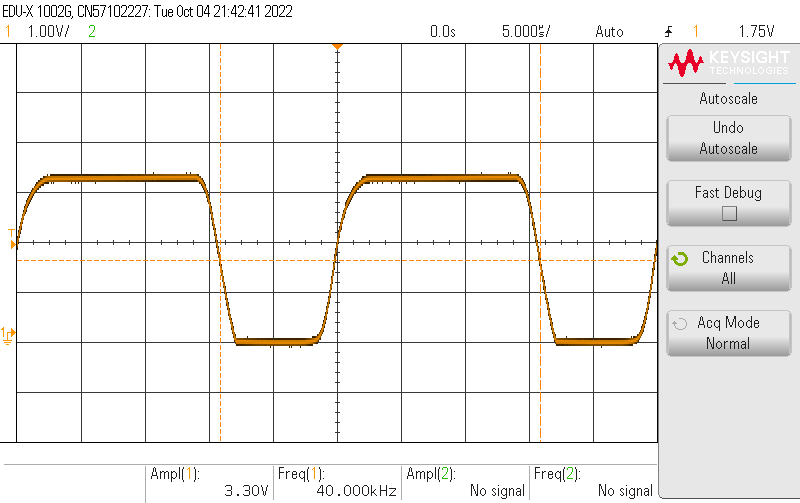
\includegraphics[width=8.5cm,height=6cm]{../Images/scope_17.png}}
        \caption{Clamped and clipped output signal.}
        \label{fig:osc-receiver-clamp-clip}
    \end{subfigure}
    \caption{Oscilloscope reading of the output voltages of the receiver circuit.}
    \label{fig:osc-receiver-3}
\end{figure}

%\section{Power Supply}

\section{Integrated System}
Once the system was integrated, the system was tested to ensure it worked correctly. To do this, an audio radar system was setup using a speaker and microphone. This setup is illustrated by the diagram in Figure~\ref{fig:audio-setup}.

\begin{figure}[htbp]
    \centering
    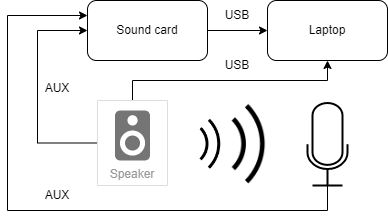
\includegraphics[width=0.6\columnwidth]{../Images/audio_setup.drawio.png}
    \caption{Setup of the audio \gls{radar} system.}
    \label{fig:audio-setup}
\end{figure}

Once the microphone and speaker are put into position, they are connected to the external sound card (XONAR U5) and the \gls{pc}. The \textsc{MATLAB} application is then run to transmit a signal of 20 kHz at a sampling rate of 44.1 kHz \footnote{It is important to note that the sampling rate satisfies the Nyquist criterion which states that the rate a signal is sampled at should be at least twice the frequency of the signal. This concept is followed for all testing and experiments carried out in this work.} for 3 seconds. It is important to note that the \gls{pc} was set to transmit sound from a single channel of the speaker - this meant only one of the two speakers was transmitting sound at any one time. The \gls{gui} shows the resulting instantaneous, average, and maximum speeds, and an output of the spectrogram and signal processing done on the received signal is shown in Figure~\ref{fig:audio-output}. For this test, a hand is moved towards the microphone (receiver), then away from it (towards the speaker), and towards the microphone again. It was expected that a hand travelling towards the microphone would result in compressed waves, resulting in a higher frequency, as the hand approaches the microphone. This effect can accurately be seen in Figure~\ref{fig:audio-speeds}.

\begin{figure}[htbp]
    \centering
    \captionsetup{type=figure}
    \begin{subfigure}[t]{0.5\textwidth}
        \centering
        \def\svgwidth{1\linewidth}
        {\scriptsize
            \setstretch{0.7} % Line spacing
            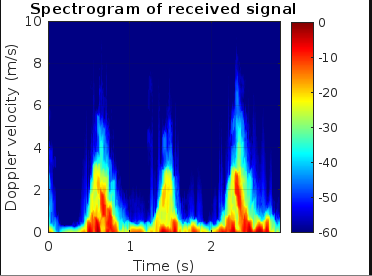
\includegraphics[width=8.5cm,height=6cm]{../Images/specTest.png}}
        \caption{Spectrogram output of moving hand for audio radar system.}
        \label{fig:audio-spectrogram}
    \end{subfigure}%
    ~ 
    \begin{subfigure}[t]{0.5\textwidth}
        \def\svgwidth{1\linewidth}
        {\scriptsize
            \setstretch{0.7} % Line spacing
            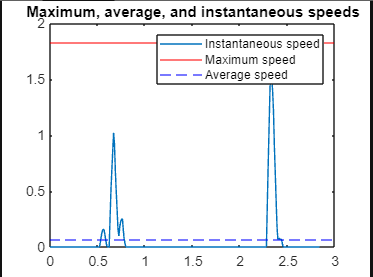
\includegraphics[width=8.5cm,height=6cm]{../Images/speedsPlot.png}}
        \caption{Output instantaneous, average, and maximum speeds of moving hand from \textsc{MATLAB} \gls{gui}.}
        \label{fig:audio-speeds}
    \end{subfigure}
    \caption{Output figures of testing audio \gls{radar} system with a moving hand.}
    \label{fig:audio-output}
\end{figure}

In Figure~\ref{fig:audio-spectrogram}, the spectrogram clearly shows the areas where the hand moves towards the microphone in the gradual rise of the signal on the plot. When the hand moves towards the speaker, lower frequencies are observed. Once it was established that the signal processing works and the \textsc{MATLAB} application effectively detected the moving hand and calculated the speeds accurately, the ultrasonic \gls{radar} system was tested in the same way and its results compared to that of the audio radar system.
% ----------------------------------------------------
\ifstandalone
\bibliography{../Bibliography/References.bib}
\printnoidxglossary[type=\acronymtype,nonumberlist]
\fi
\end{document}
% ----------------------------------------------------